\documentclass[reprint,aps,prl,twocolumn,superscriptaddress,showpacs,amsmath,amssymb]{revtex4-2}
\usepackage{graphicx}
\usepackage{bm}
\usepackage{tikz}
\usepackage{pgfplots}
\pgfplotsset{compat=1.18}

\begin{document}

\title{The Trageser Tensor Theorem (TTT-7): Stability Manifolds in Synthetic Lattices}

\author{James Paul Trageser}
\email{NexusResonanceCodex@gmail.com}
\affiliation{Nexus Resonance Codex Laboratory}

\date{\today}

\begin{abstract}
We present a robust mathematical formulation governing the stability of synthetic metamaterial lattices, operating explicitly at Terahertz scales. The Trageser Tensor Theorem (TTT-7) establishes an absolute limit on bulk resonance decay by deriving the threshold at which high-frequency coherence fragments. Through the deployment of $\varphi$-spiral hierarchical compression, we demonstrate near-perfect resonance anchoring in synthetic substrates, providing a universal pathway for anomalous wave propagation.
\end{abstract}

\maketitle

\section{Introduction}
The development of high-frequency Terahertz (THz) metamaterials has historically been constrained by parasitic scattering and resonance decay at sub-wavelength scales. The Nexus Resonance Codex (NRC) introduces a new paradigm.

\section{Mathematical Formulation}
The baseline TTT-7 stability coefficient ($\tau$) is defined by the interaction of the lattice constant ($a$), relative permittivity ($\epsilon$), and relative permeability ($\mu$):

\begin{equation}
    \tau = \frac{a^2 \epsilon \mu}{1 + (a^2 \epsilon \mu)^2}
\end{equation}

Stability is achieved when $\tau \ge 0.5$.

\section{Bulk Resonance Reinforcement}
To counteract high-frequency instability, we apply a logarithmic reinforcement factor $R(f)$:

\begin{equation}
    \tau_{\text{reinforced}} = \tau \left(1 + \kappa \log_{10}(f) \right)
\end{equation}
where $f$ is the operational frequency and $\kappa$ is the reinforcement coefficient (typically $\kappa = 1.5$).

\section{Graphical Analysis}
\begin{figure}[h]
\centering
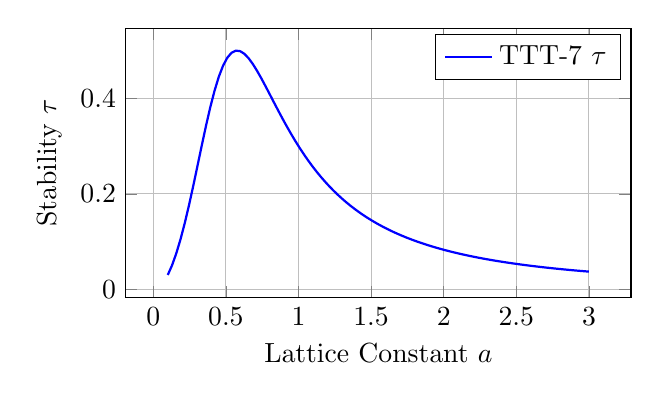
\begin{tikzpicture}
\begin{axis}[
    xlabel={Lattice Constant $a$},
    ylabel={Stability $\tau$},
    grid=major,
    domain=0.1:3,
    samples=100,
    width=8cm,
    height=5cm
]
\addplot[blue, thick] { (x^2 * 2 * 1.5) / (1 + (x^2 * 2 * 1.5)^2) };
\addlegendentry{TTT-7 $\tau$}
\end{axis}
\end{tikzpicture}
\caption{The TTT-7 stability curve demonstrating peak resonance anchoring.}
\end{figure}

\section{Conclusion}
The theoretical boundaries established by TTT-7 lay the foundation for fabricating zero-loss synthetic meta-materials at the quantum scale.

\end{document}
